% !TEX program = xelatex
\documentclass[a4paper,12pt]{article}
\usepackage{graphicx} % Required for inserting images
\usepackage[]{geometry} % Insert size in the [] to define and control the margins in the page
\usepackage{hyperref} % Makes links and table of contents clickable
% \hypersetup{colorlinks=true, linkcolor=blue} Use this if you want the links to be noticeable and have color blue, the color can be changed
% \usepackage{mathtools} % math tools builds up apon amsmath, so only one of them is needed, note that mathtools has all the function that amsmath has and even more
\usepackage{amsmath ,amssymb,amsthm}
\usepackage{tikz}
\usepackage{pgfplots}
\usepackage{float}  % Import the float package, needed to be loaded before bidi, used for positioning figures, the extreme version of [h]. Use [H] 
% ============================================================ %
% HEBREW support via polyglossia %
% ============================================================ %
\usepackage{polyglossia}
\defaultfontfeatures{Mapping=tex-text, Scale=MatchLowercase}
\setdefaultlanguage{english}
\setotherlanguage{hebrew}
\newfontfamily\hebrewfont[Script=Hebrew]{Arial}
% Use \begin{hebrew} block of text \end{hebrew} for paragraphs.
% Use \texthebrew{ } and \textenglish{ } for short texts.
% ============================================================ %
\usepackage{bidi} % we use bidi for Right-To-Left (RTL) writing
\usepackage{cancel} % Used to cancel out terms, looks different on different uses for some reason and I don't understand why
\renewcommand{\qed}{\hfill\blacksquare}
\title{\texthebrew{מאקרו א' - תרגול 0}}
\author{\texthebrew{צוות הקורס המדהים}}
\date{\texthebrew{}}
% Begin of Document ---------------------------------------- %

\begin{document}
\begin{RTL} % a command from the bidi package

    

% Title ---------------------------------------- %
\maketitle
\newpage
% Table of Contents ---------------------------------------- %
% \tableofcontents
% \newpage
% Start of paper ---------------------------------------- %
\begin{hebrew}
\section{הקדמה}
% a way to split up the chapters so the code won't be one big mess in the main.tex file
% Note that if you want to create and use commands aka shortcuts, you must define them in the main.tex file 
    מטרת התרגול הינה לחזור וללמוד כלים מתמטיים אשר נשתמש בהם בהמשך הקורס, בעיקר באמצע ובסוף
\section{מעבר בין פונקציה אקספוננציאלית לליניארית}
\begin{equation*}
    Y = 2^t
\end{equation*}
\begin{equation*}
    \ln(Y) = \ln (2^t) = t \cdot \ln(2)  
\end{equation*}
\\
\begin{tikzpicture}
    \begin{axis}[
        xlabel=$t$,
        ylabel=$Y$,
        axis lines=left,
        width=0.5\textwidth,
        height=0.5\textwidth,
        % legend pos=north east,
    ]
    
    % Exponential function
    \addplot[blue, domain=0:3, samples=100] {exp(x)};
    % \legend{$Y = 2^t$}
    
    \end{axis}
\end{tikzpicture}
\hfill
\begin{tikzpicture}
    \begin{axis}[
        xlabel=$t$,
        ylabel=$\ln(Y)$,
        axis lines=left,
        width=0.5\textwidth,
        height=0.5\textwidth,
    ]
    
    % Linear function (ln(Y))
    \addplot[red, domain=0:3, samples=100] {x};
    % \legend{$\ln(Y)$}
    
    
    \end{axis}
\end{tikzpicture}
\newpage
\section{חישובי שיעור צמיחה}
ניתן לחשב שיעורי צמיחה ב2 אופנים:
\subsection{חישוב בדיד}
חישוב זה מתאים בעיקר לתקופות זמן ארוכות, מחשבים את שיעור הצמיחה ביחס לתוצר המקורי
\begin{equation*}
    \hat Y_t = \frac{Y_t - Y_{t-1}}{Y_{t-1}}
\end{equation*}
אך יש בעיה בשיטה הזאת, אם השקעתם איי פעם בשוק ההון כנראה שאתה כבר יודעים על מה מדובר.
\\
\textbf{\textit{הבעיה:}} אין סימטרייה בין עלייה וירידה בתוצר. \\
\textbf{\textit{דוגמה:}} \\
ממלכת חזק (ידועה גם בשם חזקילנד), היא מדינה בעלת כלכלה משובחת וחזקה ונניח שהתוצר שלה הוא 100, בשנה הבאה התוצר יעלה ב50\% ולכן יהיה 150. בשנה אחריה הוא ירד ב50\% ולכן הוא יהיה 75 ולא 100.
\subsection{חישוב רציף}
בניגוד לחישוב הבדיד, חישוב זה מתאים דווקא לתקופות זמן קצרות.
\begin{equation*}
    \hat Y_t = \ln (Y_t) - \ln (Y_{t-1}) = \ln \left(\frac{Y_t}{Y_{t-1}}\right)
\end{equation*}
\textbf{\textit{דוגמה:}} \\
\begin{align*}
    \ln(11) - \ln(10) = 0.095 = 9.5\% \\
    \ln(10) - \ln(11) = -0.095 = -9.5\%
\end{align*}
סימטריות, כמה נפלא!\\
\\
\textbf{\textit{הוכחה}}:
\begin{equation*}
    \ln \left (\frac{Y_t}{Y_{t-1}} \right ) = 
    \ln \left (\frac{Y_t -Y_{t-1} + Y_{t-1}}{Y_{t-1}} \right ) = 
    \ln \left (1 + \frac{Y_t - Y_{t-1}}{Y_{t-1}} \right)
\end{equation*}
כעת נשתמש בגבול הבא ( לא לדאוג אתם לא צריכים לדעת את זה ולא צריכים לדעת להוכיח את זה ) :
\begin{equation*}
    \lim_{x \to 0} \ln (1+x) = x
\end{equation*}
לכן , ככל ש $ \dfrac{Y_t - Y_{t-1}}{Y_{t-1}}$ שואף ל 0 :
$$\ln \left (1 + \dfrac{Y_t - Y_{t-1}}{Y_{t-1}} \right) = \left (\dfrac{Y_t - Y_{t-1}}{Y_{t-1}} \right)$$
$\qed$
\newpage

\begin{table}[h!]
\centering

\begin{tabular}{|c|c|c|c|} \hline 
$t$ & $Y$ & $\ln(Y)$ & $\hat{Y}$ \\ \hline 
0 & 100 & 4.605170186 &  \\ \hline 
1 & 120 & 4.787491743 & 18.23\% \\ \hline 
2 & 140 & 4.941642423 & 15.42\% \\ \hline 
3 & 160 & 5.075173815 & 13.35\% \\ \hline 
4 & 180 & 5.192956851 & 11.78\% \\ \hline

\end{tabular}

\end{table}
בגרף לוגריתמי כמו הגרף בעמוד הראשון:
\begin{enumerate}
    \item שיפוע בין נקודות - מייצג את שיעור הצמיחה באותה שנה
    \item שיפוע בין הנקודה האחרונה לנקודה הראשונה - מייצג ממוצע צמיחה שנתי לאורך כל התקופה
\end{enumerate}
למשל,
$$\frac{5.192 - 4.605}{4 - 0} = 14.675\%$$
בנוסף לכל מה שאמרנו, גרף לוג מאפשר לנו להשוות בין מדינות שקודם לא יכלנו להשוות בניהם והוא אפילו מספק יותר מידע
\begin{figure}[H]
    \centering
    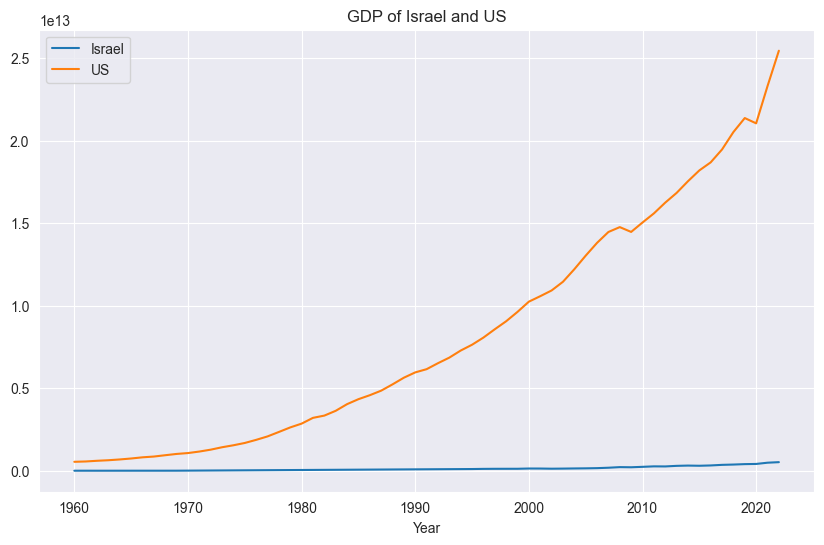
\includegraphics[width=\linewidth]{GPD - US - Israel.png}
    \caption{השווה בין תוצר ישראל ואמריקה}
\end{figure}

\begin{figure}[H]
    \centering
    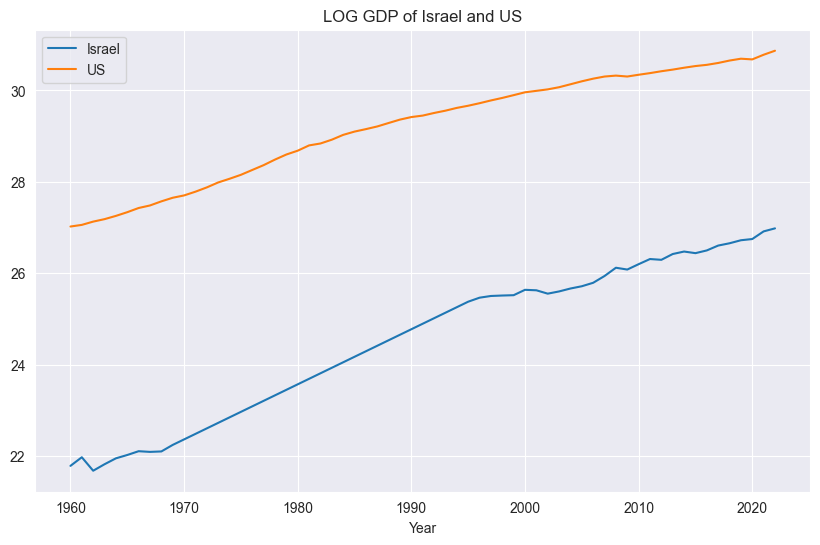
\includegraphics[width=1\linewidth]{LOG - GDP - ISRAEL - US.png}
    \caption{השווה בין לוג תוצר ישראל ואמריקה}
    
\end{figure}
\begin{figure}[H]
    \centering
    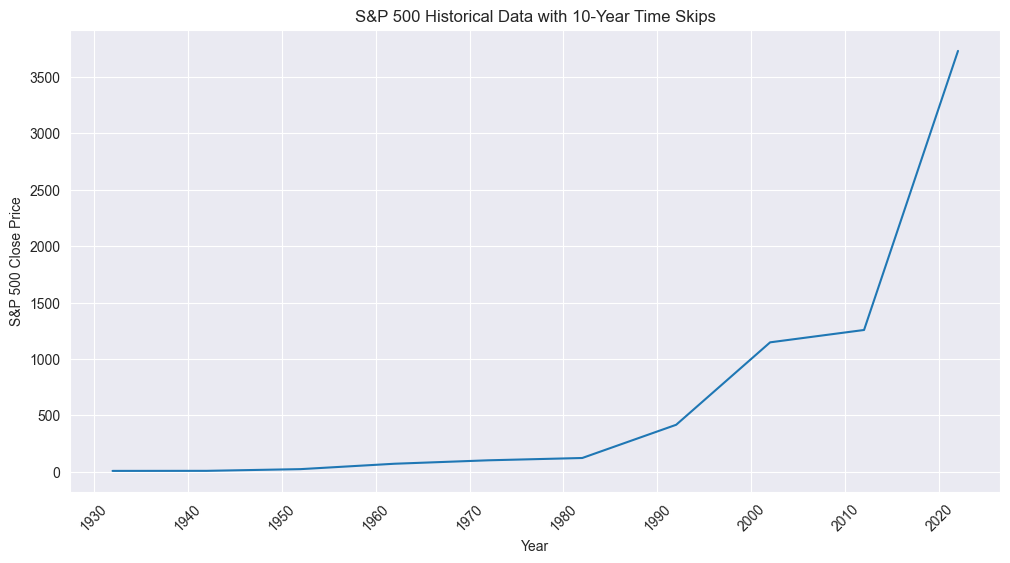
\includegraphics[width=\linewidth]{S&P500_graph.png}
    \caption{מחיר סגירה של המדד }
\end{figure}

\begin{figure}[H]
    \centering
    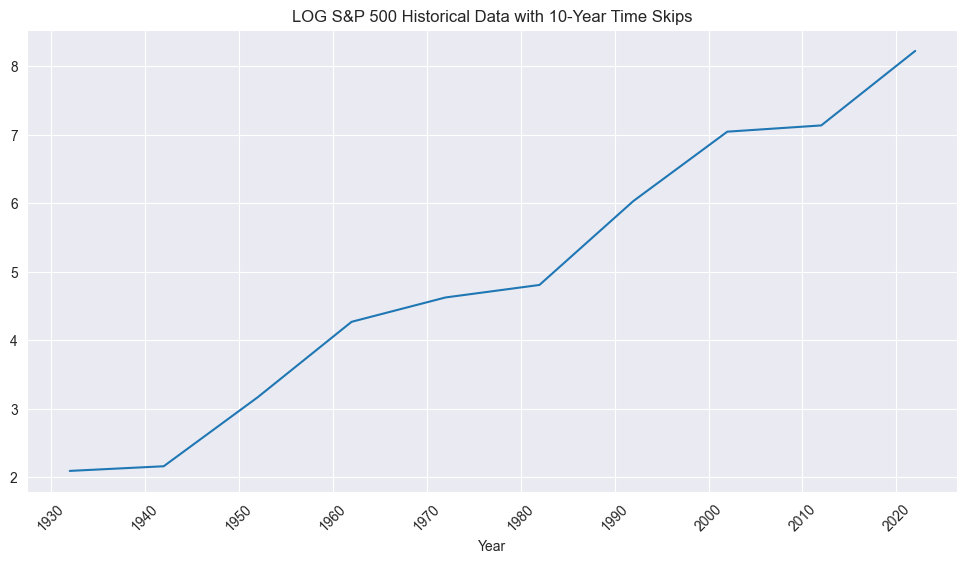
\includegraphics[width=1\linewidth]{LOG S&P500.png}
    \caption{לוג מחיר סגירה של המדד}
\end{figure}
בקורס נעסוק ביחסים בין גדלים שונים:
\begin{itemize}
    \item $\frac{Y}{N}$ תוצר לנפש
    \item $\frac{K}{Y}$ יחס הון תוצר
    \item $\frac{D}{Y}$ יחס חוב תוצר
    \item $\frac{Y}{L}$ תוצר לעובד
    \item $\frac{K}{L}$ יחס הון לעובד
\end{itemize}
גם את היחסים הללו נרצה לחקור ולראות כיצד הם משתנים לאורך זמן. לכן גם כאן נשתמש אפשר להתשמש או בחישוב בדיד או בחישוב רציף.
\\
לדוגמה ניקח את היחס תוצר לנפש $\dfrac{Y}{N}$ \\
\textbf{\textit{חישוב בדיד:}}
\begin{multline*}
\widehat{\left(\dfrac{{Y}}{N}\right)} = \dfrac{\widehat{Y}}{\widehat{N}}=\dfrac{\dfrac{Y_t}{N_t}-\dfrac{Y_{t-1}}{N_{t-1}}}{\dfrac{Y_{t-1}}{N_{t-1}}}=\dfrac{\dfrac{Y_{t-1}(1+\widehat{Y})}{N_{t-1}(1+\widehat{N})}-\dfrac{Y_{t-1}}{N_{t-1}}}{\dfrac{Y_{t-1}}{N_{t-1}}}=\dfrac{1+\widehat{Y}}{1+\widehat{N}}-1 \\
= \dfrac{1+\widehat{Y}-1-\widehat{N}}{1+\widehat{N}}=\dfrac{\widehat{Y}-\widehat{N}}{1+\widehat{N}}
\end{multline*}

אם נחלק את התקופה הזאת לעשירית תקופה, הצמיחה תהיה עשירית מהצמיחה והגידול באוכלוסיה גם יהיה עשירית מהגידול
\begin{equation*}
    \widehat{\left(\frac{Y}{N}\right)}
    = \dfrac{0.1\widehat Y - 0.1 \widehat N} {1 + 0.1\widehat N}
\end{equation*}

במידה ונרצה לחזור לתקופה המקורית, אפשר להכפיל פשוט את הגודל שקיבלנו פי 10
\begin{equation*}
    \widehat{\left(\frac{Y}{N}\right)}
    = \dfrac{10\cdot(0.1\widehat Y - 0.1 \widehat N)} {1 + 0.1\widehat N}
\end{equation*}
ומכאן קל לראות שככל שניקח תקופה קטנה יותר ככה המכנה יתכנס לאחד ונקבל כמו בחישוב רציף
\begin{equation*}
    \widehat{\left(\frac{Y}{N}\right) }= \widehat Y - \widehat N
\end{equation*}
נוכיח את התוצאה הזאת בצורה פורמלית בהמשך.
\newpage

\section{תמ''ג}
כפי שלמדתם במבוא למאקרו, תמ''ג זה תוצר מקומי גולמי. אבל חשוב להדגיש שישנם כמה סוגי תוצר,התוצר המקומי הגולמי של משק שווה לערך סך המוצרים והשירותים הסופיים שהופקו במשך שנה במשק.
כלכלנים רואים בתוצר או בתוצר לנפש, ליתר דיוק  מדד לסך רווחת הצרכנים שהופקה במהלך שנה, (למרות
הבעייתיות הרבה שבכך אינו מודד פנאי, זיהום ודברים נוספים הפוגעים ברווחה.) הסיבה שהתוצר לנפש
מהווה מדד לרווחה היא שישנה קורלציה גבוהה בעולם בין תוצר לנפש במשק לבין תוחלת החיים / תשתיות
פיסיות / כמות המזון שנהנים ממנו האזרחים ומשתנים רבים אחרים הנתפסים כמעידים על איכות חיים
גבוהה. למעשה, כלכלנים טרם הצליחו למצוא מדד טוב יותר ובמהלך הקורס נתרכז רק 2 והם:    
\begin{enumerate}
    \item תוצר נומינלי
    \item תוצר ראילי
\end{enumerate}
\begin{equation*}
    Y_{{nominal}}=\sum Y_t \cdot P_t
\end{equation*}
\begin{equation*}
    Y_{{Real}}=\sum Y_t \cdot P_0
\end{equation*}
מדידת התוצר מאפשרת לנו 2 דברים:
\begin{enumerate}

    \item להשוות בין מדינות שונות באותה תקופת זמן
    \item להשוות בין אותה מדינה לתקופות זמן שונות
\end{enumerate}

ניתן לראות שהבדל העיקרי בין ה2 הינו שתוצר נומינלי יכול לגדול בלי שהתוצר עצמו $(Y_t)$ יגדל, דבר שיכול להיות מאוד מבלבל ומטעה ובכך גורם לשימוש בתוצר נומינלי להיות לא יעיל ולא מדויק.
\\
\textbf{\textit{לדוגמה:}}
\\
\begin{figure}[H]
    \centering
    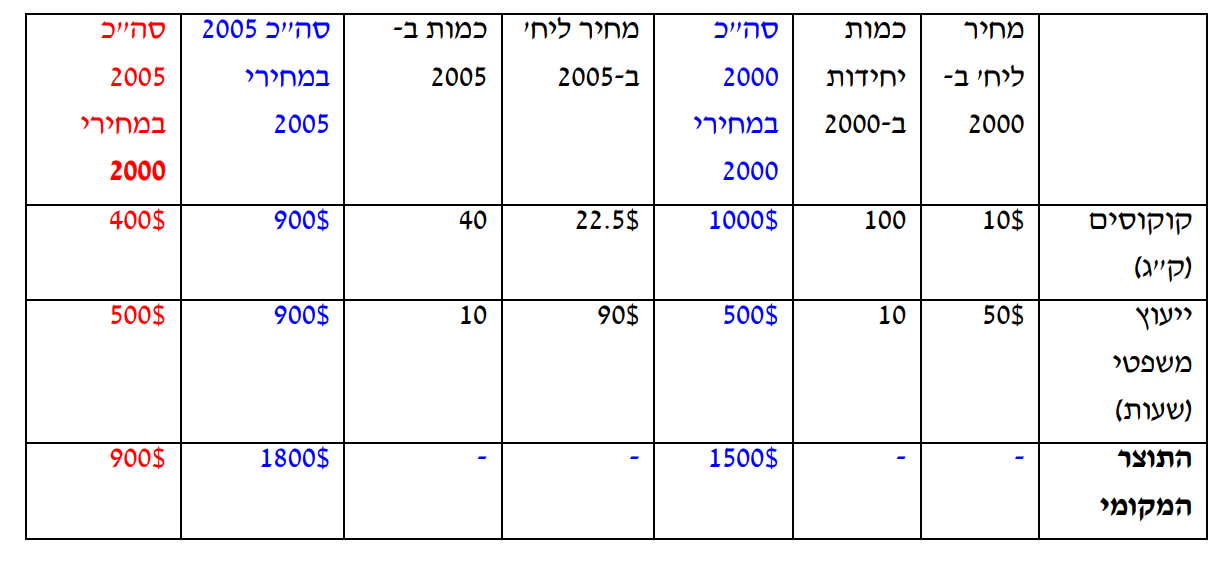
\includegraphics[width=1\linewidth]{table.png}
    \caption{כאשר מסתכלים על תוצר הנומילי אז נראה שהתוצר גדל והכלכלה התרחבה אולם כאשר מנרמלים שינוי במחירים מגלים שדווקא ההפך קרה ותוצר קטן}
\end{figure}
זהוי בדיוק הסיבה מדוע משתמשים בתוצר ריאלי, היות ואנחנו רוצים לדעת בדיוק מתי הכלכלה גדל, כלומר תוצר גדל בלי ששינוי במחירים יטעה אותנו.
על מנת להקל במעבר בין תוצר נומינלי לתוצר ריאלי נגדיר מושג חדש:
\begin{equation*}
    Deflator_t := \frac{\sum P_t \cdot Y_t}{\sum P_0 \cdot Y_t} = \frac{Y_{nominal,t}}{Y_{Real,t}}
\end{equation*}
$Deflator$ בדיוק כמו שהוא נשמע, מטרתו למחוק את השפעת האינפלציה מהתוצר ואנחנו נשתמש בו על מנת לעבור בין תוצר נומינלי וריאלי והפוך, בפרט
\begin{equation*}
    Y_{Real} \stackrel{{\textit{def}}}{=}  \sum P_0 \cdot Y_t = \frac{\sum P_t \cdot Y_t}{Deflator_t}
\end{equation*}
במילים קצת אחרות $Deflator$ מראה בכמה רמת המחירים השתנתה בשנה $t$ לעומת שנת הבסיס 0\\
\textbf{שיעור השינוי} במדד מחירי התוצר בתקופה הנוכחית ביחס לקודמת מודד את שיעור האינפלציה:
\begin{equation*}
    \widehat{Deflator_t} = \frac{Deflator_t}{Deflator_{t-1}} - 1 = \pi_t
\end{equation*}
\begin{equation*}
    \widehat{Y_t} = 
    \frac{\widehat{Y}_{nominal,t}-\widehat{Deflator_t}}{1 + \widehat{Deflator_t}} = 
    \frac{\widehat{Y_t} - \pi_t}{1+\pi_t} \approxeq 
    \widehat{Y}_{nominal,t} - \pi_t
\end{equation*}
\\
חשוב להדגיש שהקירוב נכון רק במידה והאינפלציה $\pi_t$ היא נמוכה (בערך כ1\% - 2\%), כלומר קצב הצמיחה הראלי במשק הוא ההפרש בין קצב צמיחה נומינלי ושיעור האינפלציה. \\
ניתן לראות תוצאה דומה כאשר מדברים על תוצר לנפש:
\begin{equation*}
    Y_{pc} = \frac{Y}{N} 
\end{equation*}
במידה וקצב גידול האוכלוסיה $n$ קרוב ל0 נקבל
\begin{equation*}
    \widehat{Y}_{pc} = \widehat{Y} - n 
\end{equation*}
\newpage
\section{נגזרות, כלל שרשרת ונגזרת לפי זמן}
\begin{equation*}
    \dot Y = Y_t - Y_{t-1 } = \underbrace{\Delta Y}_{\text{לפי זמן}}
\end{equation*}
\begin{equation*}
    \hat Y = \text{השינוי ב $Y$  ב \%} = \frac{Y_t - Y_{t-1}}{Y_{t-1}} = \frac{\dot Y}{Y}
\end{equation*}
\\
% \newpage
עד כה אלו היו סימונים / הגדרות שנשתמש בהם בקורס, כעת נעבור לדבר על נגזרות, ובפרט על הנגזרת של פונקצית 
 ה - $ln$, כאשר בתוך הלוג ישנו משתנה שתלוי בעצמו בזמן
\begin{equation*}
    \ln (Y(t))
\end{equation*}
אם גוזרים לפי $t$ אז יש לגזור לפי כלל שרשרת שהוא:
\begin{equation*}
\frac{d \ln (Y)}{dt} = \frac{d \ln (Y)}{dY} \cdot \frac{dY}{dt}
\end{equation*}
נשים לב לכך ש,
\begin{equation*}
    \frac{dY}{dt} = \dot Y
\end{equation*}
נציב את זה בחזרה לתוך הכלל שרשרת ממקודם ונקבל 
\begin{equation*}
    \frac{d \ln (Y)}{dt} =\underbrace{ \frac{d \ln (Y)}{dY}}_{ = \frac{1}{Y}} \cdot \  \dot Y = \frac{\dot Y }{Y} = \hat Y
\end{equation*}
בעברית, מה שקיבלנו זה שאם גוזרים לוג של תוצר לפי זמן אז מקבלים את אחוז השינוי בתוצר, תוצאה מאוד חשובה ושימושית

\section{חוקי כובע זהים לחוקי לוג}
נסמן תוצר בתור $Y$ ונסמן אוכלוסיה בתור $N$, נניח ובצדק ששני המשתנים הללו תלויים בזמן $t$. \\
\textbf{\textit{הוכחה:}} \\
לפי הגדרת הכובע
\begin{equation*}
    \widehat{ \left(\frac{Y}{N}\right)} = \dfrac{\dot{\left(\dfrac{Y}{N}\right)}}{\dfrac{Y}{N}}
\end{equation*}
תזכרו ש $\dot Y = \frac{dy}{dt}$ ולכן לפי הגדרה אפשר להפעיל אותה לוגיקה לביטוי $\frac{Y}{N}$  רק לא לשכוח שזה נגזרת של מנה היות וגם מונה וגם המכנה הם פונקציה של המשתנה שאנחנו גוזרים לפיו $t$
\begin{equation*}
\widehat{\left(\frac{Y}{N}\right)}=\dfrac{\left(\dfrac{\dot{Y}}{N}\right)}{\dfrac{Y}{N}}=\dfrac{\dfrac{\dot{Y} \cdot N-Y \cdot \dot{N}}{N^2}}{\dfrac{Y}{{N}}}=\dfrac{\dfrac{\dot{Y} \cdot N-Y \cdot \dot{N}}{N}}{Y}=\dfrac{\dot{Y} \cdot \cancel{N}}{\cancel{N} \cdot Y}-\dfrac{\cancel{Y} \cdot \dot{N}}{N \cdot \cancel{Y}}=\dfrac{\dot{Y}}{Y}-\dfrac{\dot{N}}{N}=\widehat{Y}-\widehat{N}
\end{equation*}
$\qed$
\section{זרם ומלאי}
אלו הם מושגים חשובים שנשתמש בהם במהלך הקורס וחשוב להבין את ההבדל בניהם. זרם מודד כמות המתייחסת לתקופת זמן , לדוגמה גירעון לשנת 2020. בניגוד לזרם, מלאי אינו פונקציה של זמן. לדוגמה, סך הגרעונות שהצטברו שזה למעשה החוב הציבורי. 
\begin{figure}[H]
    \centering
    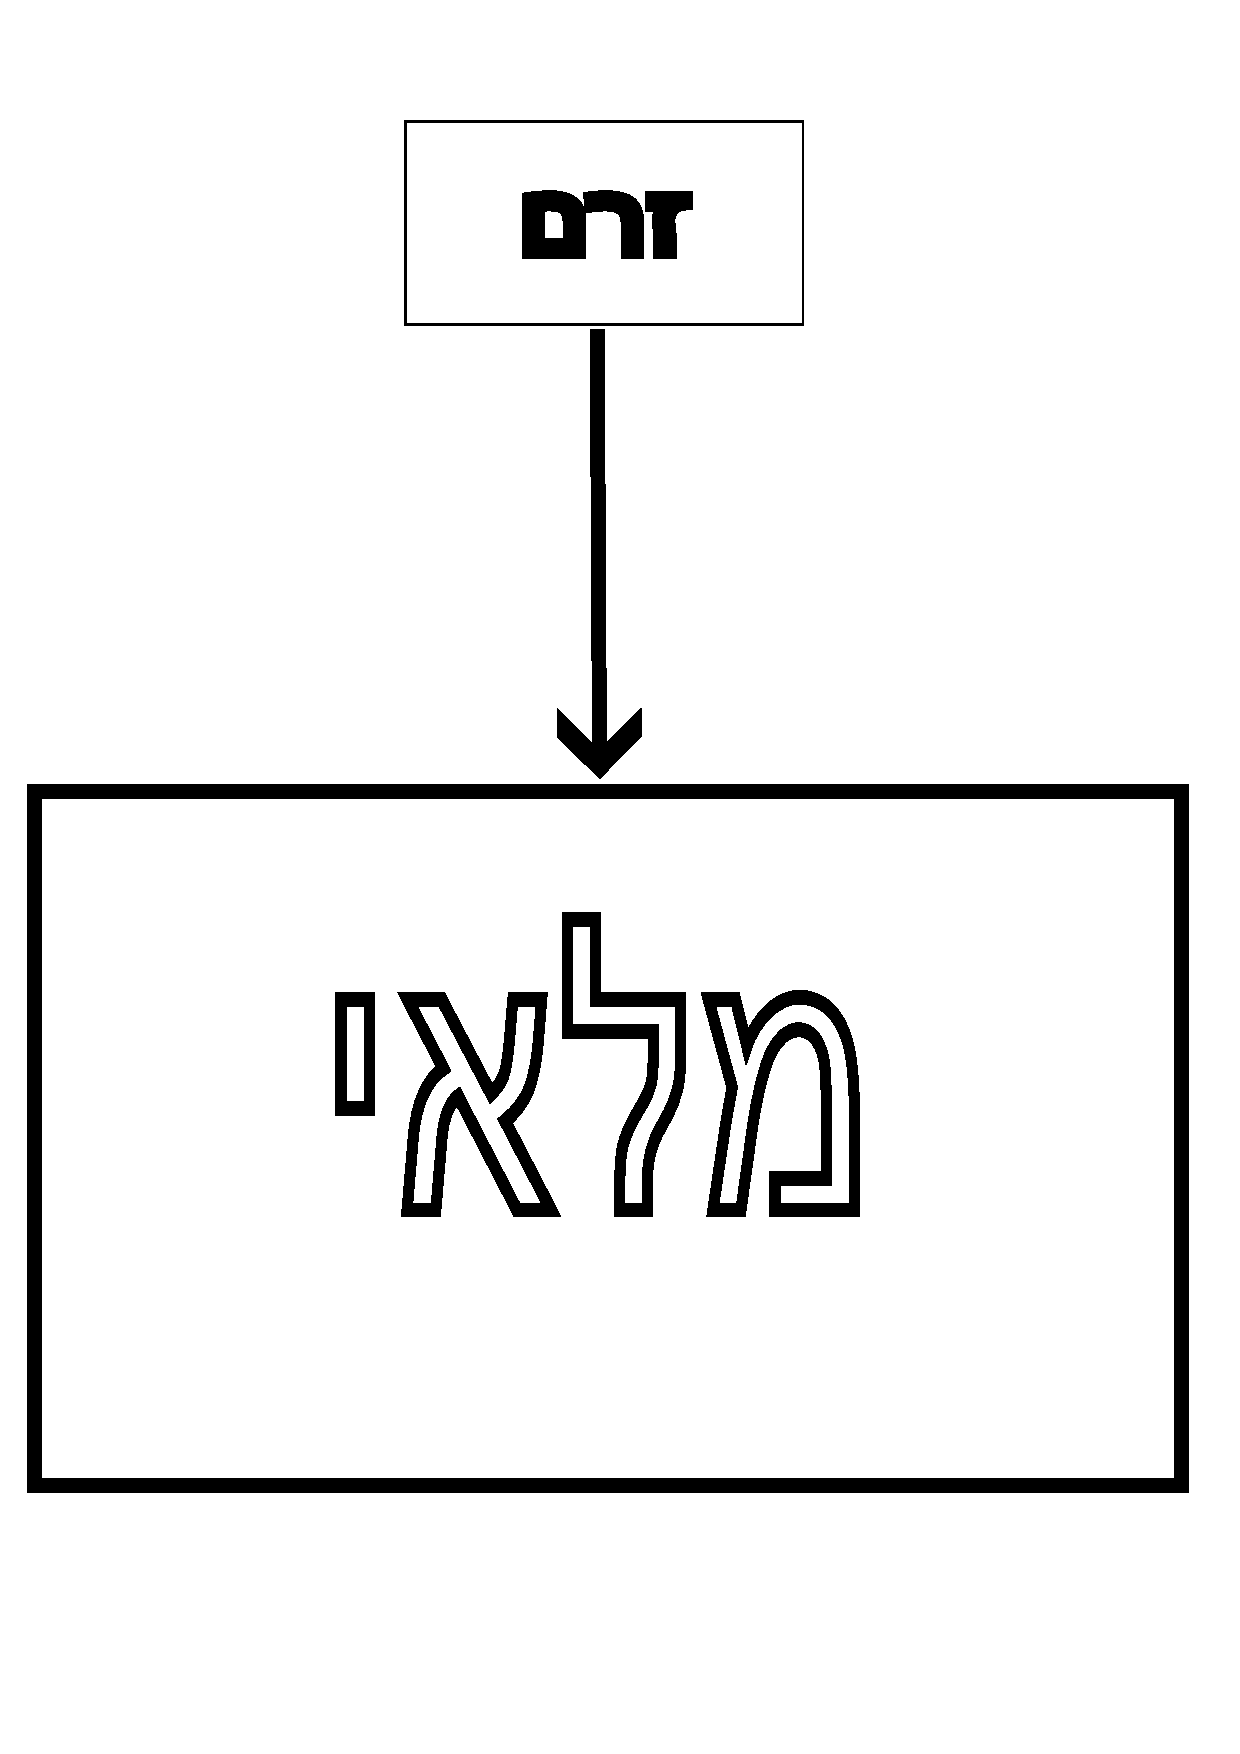
\includegraphics[width=0.5\linewidth]{drawing.pdf}
\end{figure}
\end{hebrew}    
\end{RTL}
\end{document}